% ---------------------------------------------------------------------------
%     The Flattening Lemma
%     (Seminar of Homotopy Type Theory)
%     Jonathan Prieto-Cubides
%     Universitetet i Bergen
%     Bergen, Norway
%     May 28, 2018
% ---------------------------------------------------------------------------

% ---------------------------------------------------------------------------
% -- Slides settings
% ---------------------------------------------------------------------------
\documentclass[centering]{report}
\usepackage[landscape]{geometry}
\geometry{top=0.85cm,bottom=1.4cm,left=4cm,right=4cm}
\pagestyle{empty}
\setlength{\parindent}{0pt}
% -- SLIDES PAGE NUMBERING --
\usepackage{fancyhdr}
\usepackage{lastpage}
\fancyfoot[C]{\Large\thepage/\pageref{LastPage}}
\pagestyle{fancy}
\renewcommand{\footrulewidth}{0pt}
% -- \begin{slide}...\end{slide}
\newenvironment{slide}
    {\newpage
    \vspace*{\fill}
    }
    {
     \vspace*{\fill}
    }
\newcommand{\breakslide}{\vspace*{\fill}\newpage\vspace*{\fill}}
% ---------------------------------------------------------------------------

% ---------------------------------------------------------------------------
% -- Hyperref Package
% ---------------------------------------------------------------------------

% hyperref should be loaded first as many other packages
% see https://goo.gl/Z5c9Ln
\usepackage[pagebackref,
            colorlinks,
            citecolor=darkgreen,
            linkcolor=darkgreen,
            unicode,
            pdfauthor={Jonathan Prieto-Cubides},
            pdftitle={Homotopy Type Theory Cheatsheets},
            pdfsubject={Mathematics},
            pdfkeywords={type theory, homotopy theory, univalence axiom}]{hyperref}
% ---------------------------------------------------------------------------

\usepackage[utf8]{inputenc}
\usepackage[english]{babel}

% ---------------------------------------------------------------------------
% -- Macros from the HoTT Book
% ---------------------------------------------------------------------------
\usepackage{hott}
\input{hott-book.labels}
\setcounter{secnumdepth}{1}

% ---------------------------------------------------------------------------
% -- Colors
% ---------------------------------------------------------------------------

\usepackage{color,xcolor,graphicx,overpic}
\everymath{\color{darkgreen}}

\definecolor{darkred}{rgb}{0.55, 0.0, 0.0}
\usepackage{ragged2e}
\usepackage{url}

% ---------------------------------------------------------------------------
% -- Silencing some Warning related with HoTT Labels.
% ---------------------------------------------------------------------------
\usepackage{silence}
\WarningFilter{latex}{Label}
\WarningFilter{latex}{Unused global option(s)}
\WarningFilter{latex}{There were multiply-defined labels}

\begin{document}
\Huge % -- Important for the slidess

% HoTT trick.
\setcounter{chapter}{1}
\setcounter{section}{1}

\newpage
\thispagestyle{empty}
\vspace*{\fill}
\begin{center}
  {\Huge{\underline{\textbf{The Flattening Lemma}}}} \\[4mm]
  {\Huge{(Seminar of Homotopy Type Theory)}} \\[10mm]
  {\Huge{Jonathan Prieto-Cubides}} \\[10mm]
  {\Huge Universitetet i Bergen}\\
  {\Huge Bergen, Norway}\\[20mm]
  {\Huge May 28, 2018}\\
  {\LARGE\color{gray} Updated: \today}
\end{center}
\vspace*{\fill}

\begin{slide}
\textbf{Overview}\\
\begin{itemize}
    \item Motivation
    \item The Circle
    \item Univalence and Transport
    \item The Flattening Lemma (FL)
    \item Example using FL
    \item Alternative Lemma to FL
    \item Proof of FL
\end{itemize}
\end{slide}

\begin{slide}
\textbf{Motivation:}\\

We want to prove
\begin{align*}
     \eqvspaced{\Parens{\sm{x:\Sn^1} B(x)}}{\Sn^1}
\end{align*}
where the \textbf{univalence axiom} is used to define the type family
$B : \Sn^1 \to \UU$ as follows.
\begin{mathparpagebreakable}
  B(\base) \defeq \bool
  \qquad\text{\color{black} and}\qquad
  \ap B\lloop \defid \ua(\mathsf{neg}).
\end{mathparpagebreakable}
\vspace{20mm}\\
{\color{gray}(Whiteboard. Def. of the equivalence)}
\end{slide}



% ----- The Circle
\begin{slide}
\textbf{The Circle ($\Sn^1$)}\\[3mm]
The higher inductive type $\Sn^1$ is generated by
\begin{itemize}
\item A point $\base:\Sn^1$, and
\item A path $\lloop : {\id[\Sn^1]\base\base}$.
\end{itemize}
\vspace*{5mm}
\begin{center}
  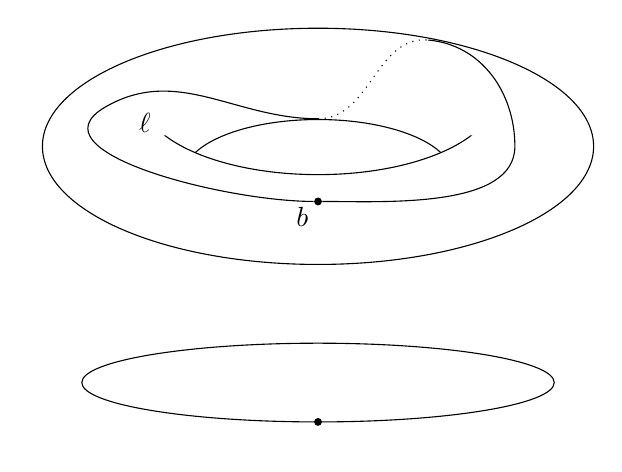
\begin{tikzpicture}
    \draw (0,0) ellipse (3 and .5);
    \draw (0,3) ellipse (3.5 and 1.5);
    \begin{scope}[yshift=4]
      \clip (-3,3) -- (-1.8,3) -- (-1.8,3.7) -- (1.8,3.7) -- (1.8,3) -- (3,3) -- (3,0) -- (-3,0) -- cycle;
      \draw[clip] (0,3.5) ellipse (2.25 and 1);
      \draw (0,2.5) ellipse (1.7 and .7);
    \end{scope}
    % \node (P) at (4.5,3) {$P$};
    % \node (S1) at (4.5,0) {$\Sn^1$};
    % \draw[->>,thick] (P) -- (S1);
    \node[fill,circle,inner sep=1pt,label={below right:$\base$}] at (0,-.5) {};
    \node at (-2.6,.6) {$\lloop$};
    \node[fill,circle,inner sep=1pt] (b) at (0,2.3) {};
    \node at (-.2,2.1) {$b$};
      \begin{scope}
        \draw (b) to[out=180,in=-150] (-2.7,3.5) to[out=30,in=180] (0,3.35);
        \draw[dotted] (0,3.35) to[out=0,in=175] (1.4,4.35);
        \draw (1.4,4.35) to[out=-5,in=90] (2.5,3) to[out=-90,in=0,looseness=.8] (b);
      \end{scope}
      \node at (-2.2, 3.3) {$\ell$};
  \end{tikzpicture}
\end{center}
\begin{lem}\label{thm:S1rec}
  \index{recursion principle!for S1@for $\Sn^1$}%
  \index{computation rule!for S1@for $\Sn^1$}%
  If $A$ is a type together with $a:A$ and $p:\id[A]aa$, then there is a
  function $f:\Sn^1\to{}A$ with
  \begin{align*}
    f(\base)&\defeq a, \\
    \apfunc f(\lloop)&\defid p.
  \end{align*}
\end{lem}
\end{slide}

\begin{slide}
The induction principle for $\Sn^1$:
\begin{itemize}
\item given $P:\Sn^1\to\type$,
\item an element $b:P(\base)$, and
\item a path $\ell : \dpath P \lloop b b$,
\end{itemize}
\begin{align*}
  \mathsf{ind}_{\Sn^1} : \sm{b:P(\base)}\, \transfib{P}{\lloop}{b} = b \to \prd{x:\Sn^1} P(x).
\end{align*}
There exists a function $f : \prd{x:\Sn^1} P(x)$ such that
\begin{align*}
f &\defeq \mathsf{ind}_{\Sn^1} (b,\ell),\\
f(\base) &\jdeq b,\\
\apd f \lloop &= \ell.
\end{align*}
\end{slide}

% -- End of the Circle ---------------------
\begin{slide}
\textbf{Univalence and Transport}

{\color{gray}
\everymath{\color{gray}}
\begin{itemize}
\item An introduction rule for {(\id[\type]{A}{B})}:
\begin{align*}
  \ua : ({\eqv A B}) \to (\id[\type]{A}{B}).
\end{align*}
\item The elimination rule for $(\id[\type]{A}{B})$:
\begin{align*}
  \idtoeqv \jdeq \transfibf{X \mapsto X} : (\id[\type]{A}{B}) \to (\eqv A B).
\end{align*}
\end{itemize}

\begin{lem}\label{thm:transport-is-ap}
  For any type family $B:A\to\type$ and $x,y:A$ with a path $p:x=y$ and $u:B(x)$, we have
  \begin{align*}
    \transfib{B}{p}{u} &= \transfib{X\mapsto X}{\apfunc{B}(p)}{u}\\
    &= \idtoeqv(\apfunc{B}(p))(u).
  \end{align*}
\end{lem}
}
\begin{lem}\label{thm:transport-is-given}
  Given $B:A\to\type$ and $x,y:A$, with a path $p:x=y$ and
  \underline{\color{black}an equivalence $e:\eqv{B(x)}{B(y)}$}
  \underline{\color{black}such that $\apfunc{B}(p) = \ua(e)$}, then for any $u:B(x)$ we have
  \begin{align*}
    \transfib{B}{p}{u} &= e(u).
  \end{align*}
\end{lem}
{\color{gray}(Pictures on the whiteboard)}
\end{slide}
% ---------

\begin{slide}
Suppose we have a type $X$ and the equivalence $e:\eqv X X$.
We can define a type family $B:\Sn^1 \to \UU$ by using $\Sn^1$-recursion:

\begin{mathparpagebreakable}
  B(\base) \defeq X
  \qquad\text{\color{black} and}\qquad
  \ap B\lloop \defid \ua(e).
\end{mathparpagebreakable}


The type $X$ thus appears as the fiber $B(\base)$ of $B$ over the basepoint. We
consider as the equivalence $e$ the boolean negation ($\mathsf{neg} :
\eqvspaced{\bool}{\bool}$). Therefore,
\vspace{3mm}
\begin{align*}
  B &\defeq \rec{\Sn^1}(\UU, \bool, \ua(\mathsf{neg})),\\
  B(\base) &\defeq \bool,\\
  B(\lloop) &:= \ua(\mathsf{neg}).
\end{align*}
{\color{gray}(Pictures on the whiteboard.)}
\end{slide}
% ---------

% \begin{equation*}
%   \xymatrixcolsep{10pc}
%   \xymatrixrowsep{5pc}
%   \vcenter{\xymatrix@1{
%       B(\base)\,\,\ar[r]^{\idtoeqv} \ar[d]_{\transfib{B(\base)}{\lloop}{\_}} &
%       \bool \ar[d]^{\mathsf{neg}}\\
%       B(\base)\ar[r]_g &
%       \bool
%       }}
%   \end{equation*}

\begin{slide}
If $x : \bool$ and $B$ as was defined above:
\begin{lem}\label{lem0}
  $\transfib{B}{\lloop}{x} = \mathsf{neg}(x).$
\end{lem}
\begin{proof}
  \cref{thm:transport-is-given} $(B, \lloop, \mathsf{neg}, x)$.
\end{proof}

{\color{gray}
\everymath{\color{gray}}
\begin{lem}\label{thm:omg}%[The $\omega$-groupoid structure of types]
  % \index{associativity!of path concatenation}%
  % \index{unit!law for path concatenation}%
  Suppose $A:\type$, that $x,y,z,w:A$ and that $p:x= y$ and $q:y = z$ and $r:z=w$.
  We have the following:
  \begin{enumerate}
  % \item $p= p\ct \refl{y}$ and $p = \refl{x} \ct p$.\label{item:omg1}
  \item $\opp{p}\ct p=  \refl{y}$ and $p\ct \opp{p}= \refl{x}$.\label{item:omg2}
  % \item $\opp{(\opp{p})}= p$.\label{item:omg3}
  % \item $p\ct (q\ct r)=  (p\ct q)\ct r$.\label{item:omg4}
  \end{enumerate}
\end{lem}


\begin{lem}\label{thm:transport-concat}
  Given $P:A\to\type$ with $p:\id[A]xy$ and $q:\id[A]yz$ while $u:P(x)$, we have
  \begin{align*}
    \trans{q}{\trans{p}{u}} = \trans{(p\ct q)}{u}.
  \end{align*}
\end{lem}
}
\begin{lem}\label{lem1}
  $\transfib{B}{\lloop^{-1}}{x} = \mathsf{neg}(x).$
\end{lem}

\begin{lem}\label{lem2}
$\transfib{B}{\lloop^2}{x} = x.$
\end{lem}
% \vfill
% \begin{center}
% 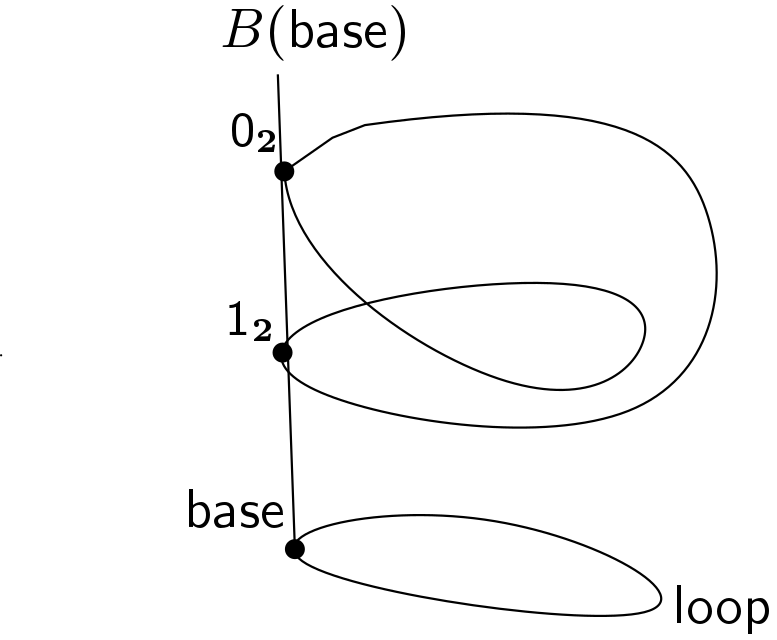
\includegraphics[width=0.7\textwidth]{Bid}
% \end{center}
% \vfill
\end{slide}
% ---------

\begin{slide}
Whiteboard.
\end{slide}
% ---------

{\color{gray}
\everymath{\color{gray}}

\begin{slide}
\begin{lem}[Dependent map]\label{lem:mapdep}
  Suppose $f:\prd{x: A} P(x)$; then we have a map
  \[\apdfunc f : \prd{p:x=y}\big(\id[P(y)]{\trans p{f(x)}}{f(y)}\big).\]
\end{lem}

\begin{lem}\label{thm:trans-trivial}
  If $P:A\to\type$ is defined by $P(x) \defeq B$ for a fixed $B:\type$, then for any $x,y:A$ and $p:x=y$ and $b:B$ we have a path
  \[ \transconst Bpb : \transfib P p b = b. \]
\end{lem}
\begin{lem}\label{thm:apd-const}
  For $f:A\to B$ and $p:\id[A]xy$, we have
  \[ \apdfunc f(p) = \transconst B p{f(x)} \ct \apfunc f (p). \]
\end{lem}
\end{slide}
% ---------

\begin{slide}
\begin{thm}\label{thm:path-sigma}
Suppose that $P:A\to\type$ is a type family over a type $A$ and let $w,w':\sm{x:A}P(x)$. Then there is an equivalence
\begin{equation*}
\eqvspaced{(w=w')}{\dsm{p:\proj{1}(w)=\proj{1}(w')} \trans{p}{\proj{2}(w)}=\proj{2}(w')}.
\end{equation*}
\end{thm}


\begin{lem}\label{eq:transport-arrow}
Given a type $X$, a path $p:\id[X]{x_1}{x_2}$, type families $A,B:X\to \type$, and a function $f : A(x_1) \to B(x_1)$,  we have
\begin{mathparpagebreakable}
  \transfib{x\mapsto A(x)\to B(x)}{p}{f} =\\
  \Big(x \mapsto \transfib{B}{p}{f(\transfib{A}{\opp p}{x})}\Big)
\end{mathparpagebreakable}
\end{lem}
\end{slide}
% ---------

\begin{slide}
\begin{thm}\label{thm:transport-path}
  For $f,g:A\to B$, with $p : \id[A]{a}{a'}$ and $q : \id[B]{f(a)}{g(a)}$, we have
  \begin{align*}
    &\id[f(a') = g(a')]{\transfib{x \mapsto \id[B]{f(x)}{g(x)}}{p}{q}}\\
    &\hspace*{60mm}{\opp{(\apfunc{f}{p})} \ct q \ct \apfunc{g}{p}}.
  \end{align*}
\end{thm}

\begin{thm}\label{thm:transport-path2}
  Let $B : A \to \type$ and $f,g : \prd{x:A} B(x)$, with $p : \id[A]{a}{a'}$ and $q : \id[B(a)]{f(a)}{g(a)}$.
  Then we have
  \begin{align*}
    &\transfib{x \mapsto \id[B(x)]{f(x)}{g(x)}}{p}{q} =\\
    &\hspace*{30mm}\opp{(\apdfunc{f}(p))} \ct \apfunc{(\transfibf{B}{p})}(q) \ct \apdfunc{g}(p).
  \end{align*}
\end{thm}
\end{slide}
% ---------
}


% -- Intro Flattening Lemma
\begin{slide}
\textbf{The Flattening Lemma}\footnote{\Large
See the full description in \cref{thm:flattening-lem}.}\\
\begin{itemize}
\item If $W$ and $\widetilde{W}$ are two higher inductive types,
\item $P : W \to \UU$ is a type family over $W$, and
\item $\widetilde{W}$ constructors can be deduced from $W$\\
constructors and from the definition of $P$
\end{itemize}
We have the equivalence
\[ \color{darkgreen} \eqvspaced{\Parens{\sm{x:W} P(x)}}{\widetilde{W}}. \]
$\widetilde{W}$ is called the ``flattened'' higher inductive
of the total space $\sm{x:W} P(x)$.
\end{slide}
% ---------

% -- The Flattening Lemma
\begin{slide}
\begin{lem}[The Flattening Lemma]
\label{thm:flattening-lem}
\begin{align*}
  \color{darkred}
  \eqvspaced{\Parens{\sm{x:W} P(x)}}{\widetilde{W}}
\end{align*}

Suppose we have $A,B:\type$ and $f,g:B\to{}A$, and that
the higher inductive type $W$ is generated by

\begin{itemize}
\item $\cc:A\to{}W$ % and
\item $\pp:\prd{b:B} (\cc(f(b))=_W\cc(g(b)))$
\end{itemize}
In addition, suppose we have
\begin{itemize}
\item $C:A\to\type$ %is a family of types over $A$, and
\item $D:\prd{b:B}\eqv{C(f(b))}{C(g(b))}$ % is a family of equivalences over $B$.
\end{itemize}
Define a type family $P : W\to\type$ recursively by
\begin{mathparpagebreakable}
  P(\cc(a)) \defeq C(a)\qquad\and{\text{\color{black}and}}\qquad
  \map{P}{\pp(b)} \defid \ua(D(b)).
\end{mathparpagebreakable}
Let \Wtil be the higher inductive type generated by
\begin{itemize}
\item $\cct:\prd{a:A} C(a) \to \Wtil$ and
\item $\ppt:\prd{b:B}{y:C(f(b))} (\cct(f(b),y)=_{\Wtil}\cct(g(b),D(b)(y)))$.
\end{itemize}
\end{lem}
\end{slide}
% ---------

\begin{slide}
\textbf{Exercise:}
\begin{align*}
\eqvspaced{\sm{x:\Sn^1}B(x)}{\Sn^1}.
\end{align*}
\begin{proof}[Solution]\ \\
We show first the equivalence,
\begin{align*}
\eqvspaced{\sm{x:\Sn^1}B(x)}{\hyperlink{suspensions}{\susp\bool}},
\end{align*}
by applying \cref{thm:flattening-lem}
with the definitions:
\begin{itemize}
\item $W \defeq\Sn^1$,
\item $A\defeq B\defeq\unit$, $f\defeq g\defeq id_{\unit}$.\\[1.5mm]
\item $\cc:\unit\rightarrow W$ with $\cc\defeq \lambda\, \_\,.\,\base$,
\item $\pp:\prd{b:\unit}\base=_{\Sn^1}\base$ with
    $\pp\defeq \lambda\, \_\,.\,\lloop$.\\[1.5mm]
\item $C: \unit\to\UU$ with $C\defeq \lambda\, \_\,.\,\bool$,
\item $D:\prd{b:B}\,\eqvspaced{\bool}{\bool}$
    with $D\defeq\lambda\, \_\,.\,\mathsf{neg}$.
\end{itemize}

\breakslide
% --------

\vspace*{\fill}
\begin{itemize}
\item The type family $P:\Sn^1\rightarrow\UU$, $P \defeq B$.
\begin{align*}
    &B(\base)\defeq\bool,\,\ \apfunc{B}(\lloop)\defeq\ua(\mathsf{neg}).
\end{align*}
\item $\Wtil\defeq\susp\bool$.\\[1.5mm]
\item $\cct : \prd{a:\unit}\bool\rightarrow\susp\bool$,\\
    $\cct \defeq \lambda \_. \rec{\bool} {(\susp\bool, \mathsf{N},\mathsf{S})}$.\\[1.5mm]
\item $\ppt:\prd{b:\unit}\prd{y:\bool}\cct(b,y)=_{\Wtil}\cct(b,\mathsf{neg}(y))$,\\
$\ppt \defeq \lambda\_.\ind{(y:\bool)}{( \mathsf{merid}(0), \opp{\mathsf{merid}(1)})}$.
\end{itemize}
In class, we proved that $\eqvspaced{\susp\bool}{\Sn^1}$.
Then, by transitivity of our equivalence relation ($\simeq$), we have
\begin{align*}
    \eqvspaced{\sm{x:\Sn^1}Bx}{\Sn^1}.
\end{align*}
\end{proof}
\end{slide}
% ---------

\begin{slide}
\textbf{Alternative Approach:\footnote{\LARGE Suggested and verified in \Agda by Håkon Robbestad}}\\

\begin{lem} For $A:\UU$, $B: A\to\UU$, $C : \UU$,
\begin{align*}
    \eqvspaced{\sm{a : A} B(a)}{C},
\end{align*}
if we have
\begin{itemize}
\item $f : \prd{a:A}(B(a)\rightarrow C)$,
\item $g : C\rightarrow A$,
\item $h : \prd{c:C}\,B(g(c))$,
\item $\boldsymbol{\alpha:\prd{c:C}\,f(g(c),h(c)) =_C c}$,
\item $\boldsymbol{\beta_0:\prd{a:A}{b:B(a)}\,g(f(a,b))=_A a}$, and
\item $\boldsymbol{\beta_1:\prd{a:A}{b:B(a)}}\\
\hspace*{35mm}\boldsymbol{\transfib{B}{\beta_{0}(a,b)}{h(f(a,b)))} = b}$.
\end{itemize}
\vspace*{\fill}
\end{lem}
\end{slide}
% ---------

\begin{slide}
\begin{proof}
Let us define
\begin{itemize}
    \item $\hat{f} : \sm{a : A} B(a) \to C$ \\ $\hat{f}((a, b)) \defeq f(a,b)$,
    \item $\opp{\hat{f}} : C \to \sm{a : A} B(a)$, \\
    $\opp{\hat{f}}(b)\defeq (g(c), h(c))$.
\end{itemize}
\begin{itemize}
    \item $s_1 : \prd{c : C} \hat{f}(\opp{\hat{f}}(c)) = c$,\\
    $s_1 \defeq \alpha$.
    \item $s_2 : \prd{(a,b) : \sm{x:A} B(x)}\, \opp{\hat{f}}(\hat{f}(a,b)) = (a,b)$,\\
    $s_2 \defeq \lambda (a,b).\opp{\text{\cref{thm:path-sigma}}}(\beta_0(a,b), \beta_1(a,b))$.
\end{itemize}
Then,
\begin{align*}
(\hat{f}, ((\opp{\hat{f}},s_1),(\opp{\hat{f}},s_2))) : \eqvspaced{\sm{a : A} B(a)}{C}.
\end{align*}
\end{proof}
\end{slide}
% ---------

\begin{slide}
\textbf{Proof of \cref{thm:flattening-lem}.} (Section 6.12 Pp. 273-289).
\begin{lem}\label{thm:flattening-cp}
  There are functions
  \begin{itemize}
  \item $\cct':\prd{a:A} C(a) \to \sm{x:W} P(x)$ and
  \item $\ppt':\prd{b:B}{y:C(f(b))} \\\hspace*{20mm}
   \Big(\cct'(f(b),y)=_{\sm{w:W}P(w)}\cct'(g(b),D(b)(y))\Big)$.
  \end{itemize}
\end{lem}
\begin{proof}\hspace{5cm}
  \begin{itemize}
    \item Define $\cct'(a,x) \defeq (\cc(a),x)$.
    \item
Given  $b:B$ and $y:C(f(b)$, since we have
\begin{align*}
\pp(b):\cc(f(b))=\cc(g(b)),
\end{align*}
\begin{align*}
 &\ppt'(b,y) : (\cc(f(b)),y) = (\cc(g(b)),D(b)(y))\\
 &\ppt'(b,y) \defeq \lambda b y.\opp{\text{\cref{thm:path-sigma}}}\\
  &\hspace{70mm}(\pp(b), \cref{thm:transport-is-given}(P,D,\pp(b),y)).
\end{align*}
  \end{itemize}
\end{proof}
\end{slide}
% ----------

\begin{slide}
\begin{lem}\label{thm:flattening-rect}
  Suppose $Q:\big(\sm{x:W} P(x)\big) \to \type$ is a type family and that we have\\[2mm]
  \begin{itemize}
  \item $c : \prd{a:A}{x:C(a)} Q(\cct'(a,x))$ and
  \item $p : \prd{b:B}{y:C(f(b))}\\
  \hspace*{20mm}\Big(\trans{\ppt'(b,y)}{c(f(b),y)} = c(g(b),D(b)(y))\Big)$. %_{Q(\cct'(g(b),D(b)(y)))}
  \end{itemize}
  \vspace*{2mm}
  Then there exists $k:\prd{z:\sm{w:W} P(w)} Q(z)$ such that $k(\cct'(a,x)) \jdeq c(a,x)$.
\end{lem}
\begin{proof} Proof in the book, Pp. 276-277.
\end{proof}
\end{slide}
% ---------

\begin{slide}
\begin{lem}\label{thm:flattening-rectnd}
  Suppose $Q$ is a type and that we have\\[2mm]
  \begin{itemize}
  \item $c : \prd{a:A} C(a) \to Q$ and
  \item $p : \prd{b:B}{y:C(f(b))}\\
  \hspace*{20mm}\Big(c(f(b),y) =_Q c(g(b),D(b)(y))\Big)$.
  \end{itemize}
  \vspace*{2mm}
  Then there exists $k:\big(\sm{w:W} P(w)\big) \to Q$ such that $k(\cct'(a,x)) \jdeq c(a,x)$.
\end{lem}
\begin{proof} Proof in the book, Pp. 277-278.
\end{proof}
\end{slide}
% ---------


\begin{slide}
\begin{lem}\label{thm:ap-sigma-rect-path-pair}
  Let $B:X\to\type$ be a type family and let
  \begin{align*}f:\sm{x:X} B(x) \to Z\end{align*}
  be defined componentwise by $f(x,b) \defeq d(x)(b)$ for a curried function $d:\prd{x:X} B(x)\to Z$.
  Then if we have
  \begin{itemize}
  \item $s:\id[X]{x_1}{x_2}$,
  \item $b_1:B(x_1), b_2:B(x_2)$, and
  \item $r:\trans{s}{b_1}=b_2$,
  \end{itemize}

 the path
  \begin{align*}
    \apfunc f (\pairpath(s,r)) :f(x_1,b_1) = f(x_2,b_2)
  \end{align*}
  is equal to the composite \dots

\breakslide
% ---------

{\color{gray}
\everymath{\color{gray}}
the path
  \begin{align*}
    \apfunc f (\pairpath(s,r)) :f(x_1,b_1) = f(x_2,b_2)
  \end{align*}
  is equal to the composite \dots
}
{\LARGE
  \begin{align}
    f(x_1,b_1)
    &\jdeq d(x_1)(b_1) \notag\\
    &= \transfib{x\mapsto Z}{s}{d(x_1)(b_1)}
    \tag{by $\opp{\text{(\cref{thm:trans-trivial})}}$}\\
    &= \transfib{x\mapsto Z}{s}{d(x_1)(\trans{(\refl{x_2})}{b_1})}
    \tag{by $\opp{\text{(\cref{thm:trans-trivial})}}$}\\
    &= \transfib{x\mapsto Z}{s}{d(x_1)(\trans{(\opp s\ct s)}{b_1})}
    \tag{by $\opp{\text{(\cref{thm:omg}\ref{item:omg2})}}$}\\
    &= \transfib{x\mapsto Z}{s}{d(x_1)(\trans{\opp s}{\trans{s}{b_1}})}
    \tag{by $\opp{\text{(\cref{thm:transport-concat})}}$}\\
    &= \big(\transfib{x\mapsto (B(x)\to Z)}{s}{d(x_1)}\big)(\trans{s}{b_1})
    \tag{by~\eqref{eq:transport-arrow}}\\
    &= d(x_2)(\trans{s}{b_1})
    \tag{by $\happly(\apdfunc{d}(s))(\trans{s}{b_1}$}\\
    &= d(x_2)(b_2)
    \tag{by $\apfunc{d(x_2)}(r)$}\\
    &\jdeq f(x_2,b_2).
    \notag
  \end{align}
  }
\end{lem}
\vspace*{5mm}
\begin{lem}\label{thm:flattening-rectnd-beta-ppt}
  $\apfunc{f}(\ppt'(b,y)) = p(b,y)$.
\end{lem}
\end{slide}
% ---------

\begin{slide}
\begin{proof}[Proof of \cref{thm:flattening-lem} (The Flattening Lemma)]
\hspace*{5cm}\\
Let us define
\begin{itemize}
    \item $k:(\sm{w:W}P(w)) \to \Wtil$ by using the recursion
    principle of \cref{thm:flattening-rectnd}, with $\cct$ and
    $\ppt$ as input data.

    \item $h:\Wtil \to \sm{w:W}P(w)$ by using the recursion principle
    for \Wtil, with $\cct'$ and $\ppt'$ as input data.
\vspace*{\fill}
\newpage
\vspace*{\fill}
    \item $s_1 : \prd{z : \Wtil} k(h(z)) = z$\\
    By induction on $z$, it suffices to consider the two constructors of \Wtil.
  But we have
  \begin{align*}
    k(h(\cct(a,x))) \jdeq k(\cct'(a,x)) \jdeq \cct(a,x)
  \end{align*}
  by definition, while similarly
  \begin{align*}
  \ap k{\ap h{\ppt(b,y)}} = \ap k{\ppt'(b,y)} = \ppt(b,y)
  \end{align*}
  using the propositional computation rule for $\Wtil$ and \cref{thm:flattening-rectnd-beta-ppt}.

  \item  $s_2 : \prd{z : \sm{w:W}P(w)} h(k(z)) = z$.\\
  But this is essentially identical, using \cref{thm:flattening-rect}
  for ``induction on $\sm{w:W}P(w)$'' and the same computation rules.
  \end{itemize}
\end{proof}
\end{slide}
% ---------

% ---------------------------------------------------------------------
% -- References --
% ---------------------------------------------------------------------
\begin{slide}
\textbf{\color{darkred} References}
\begin{itemize}
\item Univalent Foundations Program, The (2013). Homotopy Type Theory:
Univalent Foundations of Mathematics. Institute for Advanced Study.\\ URL:~\url{http://saunders.phil.cmu.edu/book/hott-online.pdf}
\item Bezem M. Lecture notes for a seminar on Homotopy Type Theory.
URL:~\url{https://github.com/marcbezem/INF329}
\end{itemize}
\end{slide}
% ---------

\begin{slide}
(Bonus Slides)
\end{slide}
% ---------


\begin{slide}
\label{sigmatype}
\textbf{Dependent pair types (\texorpdfstring{$\Sigma$}{Σ}-types)}\\[2mm]

% Judgments concerning such expressions are introduced by the following
% rules:
%
\begin{itemize}
\item if $A:\UU_n$ and $B: A \rightarrow \UU_n$, then $\sm{x:A}B(x) : \UU_n$
\item if, in addition, $a:A$ and $b:B(a)$, then $\tup a b:\sm{x:A}B(x)$
\end{itemize}
%
If we have $A$ and $B$ as above, $C : (\sm{x:A}B(x)) \rightarrow \UU_m$, and
\[
  d:\tprd{x:A}{y:B(x)} C(\tup x y)
\]
we can introduce a defined constant
\[
  f:\tprd{p:\sm{x:A}B(x)} C(p)
\]
with the defining equation
\[
  f(\tup x y)\defeq d(x,y).
\]
\end{slide}
% ---------

\begin{slide}
\label{suspensions}
\textbf{Suspensions}\\
It is a type $\susp A$ defined by the following generators:

\begin{itemize}
\item a point $\north:\susp A$,
\item a point $\south:\susp A$, and
\item a function $\merid:A \to (\id[\susp A]\north\south)$.
\end{itemize}

The recursion principle for $\susp A$ says that given a
type $B$ together with
\begin{itemize}
\item points $n,s:B$ and
\item a function $m:A \to (n=s)$,
\end{itemize}
we have a function $f:\susp A \to B$ such that $f(\north)\jdeq n$
and $f(\south)\jdeq s$, and
for all $a:A$ we have $\ap f {\merid(a)} = m(a)$.
\index{induction principle!for suspension}%
\end{slide}
% ---------

\begin{slide}
Similarly, the induction principle says that given
$P:\susp A \to \type$ together with
\begin{itemize}
\item a point $n:P(\north)$,
\item a point $s:P(\south)$, and
\item for each $a:A$, a path $m(a):\dpath P{\merid(a)}ns$,
\end{itemize}
there exists a function $f:\prd{x:\susp A} P(x)$ such that
$f(\north)\jdeq n$ and $f(\south)\jdeq s$ and for each $a:A$
we have $\apd f {\merid(a)} = m(a)$.
\end{slide}
% ---------

\end{document}
